\section{Literature Review}

\subsection{Video games and Serious Games}

Baranowski et al \cite{yuserious} define games as a physical or mental contest with a goal or objective, played according to a framework, or rule, that determines what a player can or cannot do inside a game world. The definition covers the setup of a game, while a physical or mental contest, played according to specific rules, with the goal of amusing or rewarding the participant the reward aspect of games.

Video games are built on top of these core values with the addition of having the game world confined to some sort of digital medium. The first video game was created by William Higinbotham; it was a tennis game to be played on a television set\cite{stanton2015brief}. From the early days of video games, their main aim was always to provide some degree of entertainment. The entertainment value is achieved in various ways depending on the gaming platform, game genre and the target audience. Modern video games are simply made up of three fundamental components: story, art and software \cite{zyda2005visual}.

Moving on to serious games this type of games are considered a mix of simulation and game to improve eduction \cite{abt1970}. The idea behind a serious game is to connect a serious purpose to knowledge and technologies from the video game industry\cite{michael2005serious}. The boundaries of serious games are debated, mostly due to the fact that serious games attract multiple domains making it hard to come up with a common boundary. However, the common denominator across all domains seems to be serious game designers use people's interest in video games to capture their attention for a variety of purposes that go beyond pure entertainment\cite{djaouti2011classifying}.

The main contrast between video games and serious games is the use of pedagogic activities which aim to educate or instruct knowledge or skill \cite{zyda2005visual} in serious games as opposed to the pure leisurely aspects of the video game. Pedagogy is given preference over the amusement value which in some cases might not be found in serious games \cite{zyda2005visual}. All serious games involve learning, whether eye hand coordination skills, visual-spatial skills,  which buttons to push or what to do in a certain scenario. This is the fundamental difference between serious and entertainment games. Serious games need to educate the player with a specific type of content, whereas entertainment games need to entertain the player with whatever; racing, puzzles, it does not really matter, as long as the player enjoys it\cite{Harteveld2007}. With an entertainment game, development's main objective is too make the game fun, the content and controls should be at the service of making the game entertaining, On the other hand, serious game designers  have multiple objectives, they still need to create a compelling and fun game, but also an educating and realistic game.  From this it follows that three aspects as essential for a serious game, fun, learning and validity \cite{Harteveld2007}. One should not forget that a serious game is fundamentally a game, and a game should be fun. The game should make use of pedagogical methods and theories to ensure knowledge can be conveyed. Validity is related to the content which is being tackled in the serious game. The content which is being taught should teach relevant content that can be applied outside of the game world.

\subsubsection{Pedagogy}
In order to produce a valid pedagogical experience aspects as learning objectives, target groups and challenges needs to be clearly identified before designing a serious game\cite{moser2002methodology}. Various pedagogy theories exist which can be applied to a serious game, some of which are behaviorism, cognitivism, constructivism and situated learning\cite{egenfeldt2005beyond}. From each of these theories one can extract some important properties. 

Experience, games tend to provide learning-by-doing, Many games make use of pop-up windows with extensive amount of text that are supposed to have educational value. This technique could provide too much information, time pressure or other factors inside a game environment which could potentially lead to cognitive overload or lead a person to filtering out critical information\cite{egenfeldt2005beyond}.

Exploration. An important property of a game is that of requiring an active, participative attitude of the learner. The game world, including rules, mechanics and environment need to be explored and discovered by the learner. Many poorly designed games force the player to do something, while they should just let the player figure it out or at least guide the player into doing so.

Incremental. The learning process should occur incrementally as it will otherwise be too demanding for a player, and that is the way the human brain functions. Humans acquire knowledge piece for piece and try to integrate this into existing structures\cite{moser2002methodology}.

Deciding on a pedagogy is no easy task, one must take into account the aims and objective which is the pedagogy task is trying to achieve while also considering any capabilities and limitations the target audience might have. Such consideration must be made when designing the way information is channelled back to the user. Three main channels are considered, auditory, visual and kinaesthetic. The choice of which to use relies heavily on the domain and the end user. Some instructions might be able to be better conveyed through visual cues, while other work better as auditory or kinaesthetic, however, previous work found out that a mix of channels work better as one can compliment the other\cite{leahy2003auditory}. Such cases include instances in which timing is a factor, having a visual image further explained with audio or vice versa. A further consideration has to be made when applying this to the vehicle driving context, it is important avoid or at least minimise the effect such channels might have on the concentration of the driver. The driver is already focusing by keeping eyes on the road, usually focusing on the centre of the road ahead also keeping in the look out with rapid eye glancing at any obstacles in the vehicle surrounding area and staying attentive for any auditory cues coming from the environment which could highlight any danger\cite{engstrom2005effects}. 

\subsection{Sim Racing as a Serious Game}

Simulation racing games (sim racing) such as Asseto Corsa \cite{assestoCorsa} and Project CARS \cite{ProjectCars} , which are off-the-shelf products, provide a sim racing experience within budget for the average video game consumer. The aim with such games is to replicate real life cars, race car dynamics and track locations to amuse and entertain the player. The challenge aspect is achieved by pitting the user against other computer drivers known as AI players, or in multiplayer online races, which are played against other human players. In some cases, a user can compete against oneself by taking on a ghost - a recording of the player's best lap for a particular track. Sim racing the definition of what a video game is however, they miss the pedagogy activities which would qualify them as serious games. Most of the modern sim racing games do aid the player to improve by means of implementing aids. Such aids might include showing the racing line while also highlighting the braking and acceleration points. Other aids include anti lock brakes, traction control and stability control, these are implemented in a passive way. With the exception of the racing line, the player is not told when and what is being done wrong. This results in users having to figure out their own mistakes by means of practicing without any guidance or feedback from with the game. This final year project aims to implement a module which is plugged into an off the shelf racing simulator which. This module trains users by letting them know what is being done wrong, when it's being done wrong and most importantly how to avoid making the same mistake. Further more this project builds on the premise put forward which shows that users are able to learn road driving skills into a virtual world and then successfully applying them to the real world\cite{li2015can}\cite{vogel2006computer}. Although studies have been carried out involving training for road drivers, none have looked into teaching on racing circuits with the aim of improving racing and car handling techniques. 

\newpage
\section{Background Work}

\subsection{Motorsport racing}

In sports individuals or groups compete to be first to achieve a particular objective. In the case of circuit motorsport races, in which motorised vehicles go round a course. Each racing discipline or series has its own rules. However, at the core, all disciplines participants aim to complete a full lap of the circuit in the least amount of time. Some disciplines focus on achieving one fast lap, such as time trials, while others focus on achieving the least amount of time across a fixed amount of laps, such as FIA's Formula 1 series. This dissertation will focus on confined car racing taking place on smooth asphalt surfaces in purpose built race tracks. 

A race driver needs to figure out how to go round a piece of asphalt in the minimum amount of time \cite{GoingFaster}. In order to do so, he or she needs to develop techniques for more advanced vehicle control. One such technique is that of mastering the race line, which is considered the the fundamental skill a race driver must understand and master before moving on to anything else \cite{GoingFaster}. The racing line is the best path through a circuit, it is the path which takes the least time while keeping the higher average speed \cite{beckman1991physics}. The trickiest part of the racing line to master is that of a corner, this task is  split into two parts, identifying the line which should be taken and staying on the line. The first part refers to being able to visualise the racing line while the later refers to actually being able to control the car so that it stays on the line. Once the driver has an idea of the race line which the corner should be taken at, he or she must further split the line into three sections. The first part is the braking part, during this part the driver needs to decelerate in preparation for the corner, this is usually carried out in a straight line and end right before the turn in point. The turn in point refers to a point on the corner race line in which steering input is applied, allowing the car to turn into the corner. The turn in motion should be a smooth one, taking the car all through the corner without having to do too much corrections to the steering. The aim of the turn in section is to aim for the apex point, this is the inside middle point of the corner. The final part of tackling a corner is the acceleration part, after the apex point, the driver must start to gradually accelerate out of the corner while still turning out of the corner aiming for the outside apex.

\begin{figure}[!htb]
	\centering
	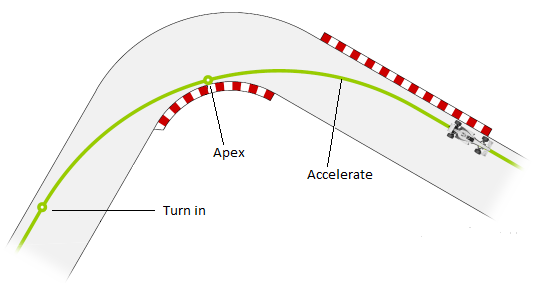
\includegraphics[height=7cm]{images/cornerraceline}
	\caption{Race line through a 90" right corner}
	\label{fig:CornerRaceLine}
\end{figure}

After the driver manages to drive the race line at a relatively slow speed, the driver must find the limit of the car. This is the maximum speed the car can be driven while still allowing the driver to have maximum control over the car. Various studies have been carried out to define such a limit in terms of the physical properties of the car and environment around it. The most important property is the level of grip the car can achieve and sustain on track. Various factors contribute to the level of grip, most notable are the tires which the car is being driven on, as the tires are the only actual contact to the track, allowing for braking, accelerating and turning forces to be transferred to the asphalt.

Each tire has two properties which are of particular interest to a drive, the slip angle and slip ratio. The slip angle is the angle between a tire’s direction of travel and the actual direction the tire is going towards. Given both the actual direction of travel and desired direction of travel are known, it becomes trivial to calculate the angle which is done by calculating the arch of the two vectors as shown in \ref{fig:slipangle}.

\begin{figure}[!htb]
	\centering
	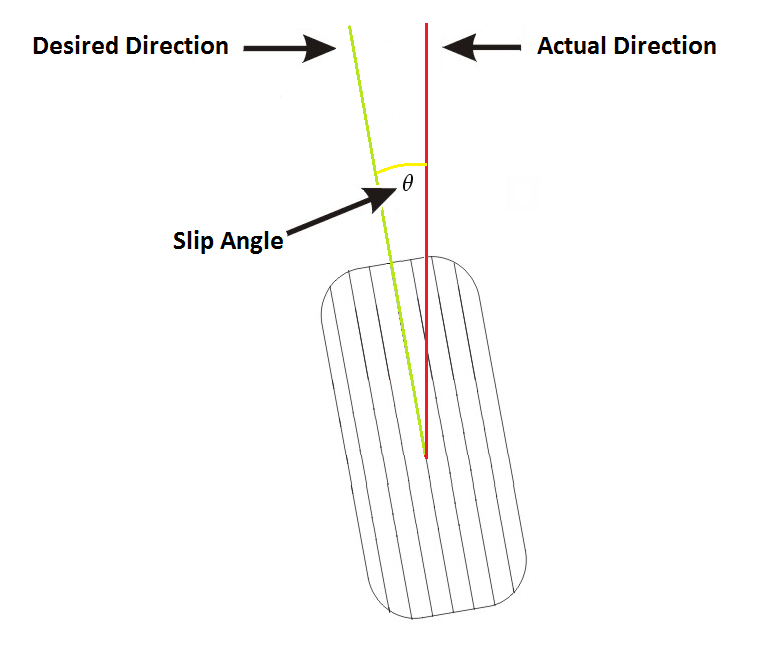
\includegraphics[height=7cm]{images/slipangle}
	\caption{Slip Angle of a tire understeering while turning left}
	\label{fig:slipangle}
\end{figure}

Whenever the slip angle is above 0’ the tire is described as being in an understeering situation. Symptoms include Light steering, drifting towards the outside of a bend and possible tyre noise from the wheels. Assuming the tires are not damaged and the track is not wet nor dirty, understeer can be caused by active factors such as cornering speed throttle, braking, steering inputs and weight transfer. Other passive factors such as Weight distribution, drive layout, suspension and chassis setup, tyre type, wear and pressures also effect understeer. An understeer situation in a corner can be avoided by not entering too fast into a corner, not accelerating too aggressively in a corner, not braking through a corner, and not making any sudden changes which drastically upset the weight distribution of the car. Passive factors have to do with the way a car is mechanically setup, such factors will be taken in consideration during this project but will not be given great importance as this project aims to improve the drive’s skills. The project will focus on the active factors as these are the ones which the driver has direct input on while driving a car. It is known for a tire to have an optimal slip angle, this is the slip angle at which the tire can produce the most grip while cornering. A comon road tire’s optimal slip angle is of 5’ while a slick tire which is purpose built for racing has an optimal slip angle of 8’-10’. These values may vary a bit depending on the tire brand\cite{beckman1991physics}

Moving on to oversteer, this is an other issue which can arise from lack of grip. Whereas understeer is caused by lack of grip in the front tires, oversteer is caused by lack of grip on the rear tires. Symptoms of oversteer include having the rear of the vehicle becoming unstable and 'light' and the car starts to rotate so the driver is facing towards the inside of the corner. Active factors causing oversteer are cornering speed, throttle, braking, steering inputs and weight transfer. The driver can avoid oversteer by not braking while in a corner and not accelerating too hard in a rear wheel drive as it makes the rear tires spin too fast, losing traction with the road.

During acceleration and braking the tire experiences rotational forces, however these rotational forces do not match the expected velocity, this means at all time there is some level of slip occurring between the tire and the road beneath it. This slip is called slip ratio and is expressed in percentage. A slip percentage of 100\% would mean the tire is rotating, but the road is stationary, this is called a burnout or wheel spin. On the other hand, a percentage of -100\% would mean the tire is not rotating but the road beneath it is moving, this can occur while braking hard and is called locking the wheels\cite{pacejka2006tire}. While braking the driver must make sure not lock up the tires as this will cause the tires to wear out quicker while also drastically increasing the stopping distance. On the other hand braking too lightly will make the car take longer to decelerate with makes the driver lose time. In order to braking optimally the slip ratio should be between 10\% to 15\% \cite{GoingFaster}.

Professional racing rigs
the likely users of the system,
the anticipated benefits of the system,





